% Operators
% =========
\RequirePackage{textcomp}
\RequirePackage{amsmath}
\RequirePackage{graphicx}
\RequirePackage{stmaryrd}

% Tree parallel
\newcommand{\tpar}{\mathbin\otimes}
% Tree label
\newcommand{\tlab}[2]{{#1}[ #2 ]}
% Sequence concatenation
\newcommand{\scat}{\mathbin\cdot}
% Heap cell
\newcommand{\cell}[2]{#1 \mapsto #2}
% Heap combination
\newcommand{\hsep}{\mathbin\ast}
% Empty heap
\newcommand{\hemp}{\mathord\mathrm{emp}}
% List cell
\newcommand{\lcell}[2]{#1 \Mapsto #2}
\newcommand{\lcellc}[2]{\lcell{#1}{\left[ #2 \right]}}

% Context application
\newcommand{\app}{\bullet}
% Context composition
\newcommand{\comp}{\circ}
% Multi-holed composition
\makeatletter
\def\moverlay{\mathpalette\mov@rlay}
\def\mov@rlay#1#2{\leavevmode\vtop{%
\baselineskip\z@skip \lineskiplimit-\maxdimen
\ialign{\hfil$#1##$\hfil\cr#2\crcr}}}
\makeatother
\newcommand{\mcc}[1]{\mathrel{\moverlay{\bigcirc\cr \raisebox{0.2ex}{$\scriptstyle{#1}$}}}}
% Substitution
\newcommand{\subs}[2]{[#1 / #2]}

% Identity of a context algebra
\newcommand{\cid}{\mathbf{I}}
% Zero of a context algebra
\newcommand{\czero}{\mathbf{0}}

% Holes function
\DeclareMathOperator{\holes}{holes}
\DeclareMathOperator{\dom}{dom}
\DeclareMathOperator{\range}{range}
\DeclareMathOperator{\freevars}{fv}

% Fresh
\newcommand{\fresh}{\mathrel{\sharp}}

%%%% Mathematics
% Partial function
\newcommand{\pfun}{⇀}
% Finite partial function
\newcommand{\fpfun}{\pfun_{\mathrm{fin}}}

% (Partial) function update
\newcommand{\fupd}[3]{{#1}[#2 \mapsto #3]}

% Powerset
\newcommand{\powset}[1]{\mathcal{P}(#1)}
\newcommand{\fpowset}[1]{\mathcal{P}_\mathrm{fin}(#1)}
% Set
\newcommand{\Set}[1]{\left\{#1\right\}}
% Set builder
\newcommand{\Setb}[2]{\left\{#1 \ \middle| \ #2 \right\}}
% Union
\newcommand{\union}{\cup}
% Intersection
\newcommand{\intersect}{\cap}
% Cardinality
\newcommand{\Card}[1]{\left|#1\right|}
% Disjoint union
\newcommand{\disjunion}{\uplus}

% Family
\newcommand{\Family}[3]{\left\{ {#1}_{#3} \right\}_{ {#3} \in {#2} }}
% Alternate macro
\newcommand{\family}[3]{\left\{ #1 \right\}_{#2 \in #3}}

% Relation composition
\newcommand{\randthen}{\mathbin{\fatsemi}}

%%%% Logical formulae

% Tree zero
\newcommand{\Ftzero}{\mathbf{0}}
% Tree parallel
\newcommand{\Ftpar}{\tpar}
% Tree label
\newcommand{\Ftlab}[2]{\tlab{#1}{#2}}
% Sequence concatenation
\newcommand{\Fscat}{\scat}

% Application
\newcommand{\Fapp}{\mathbin\bullet}
% Application adjoint (tree formula)
\newcommand{\Fappr}{\mathbin{\Fapp\!-}}
% Application adjoint (context formula)
\newcommand{\Frapp}{\mathbin{-\!\Fapp}}
% Existential versions of adjoints
\newcommand{\FapprE}{\Fappr^\exists}
\newcommand{\FrappE}{\Frapp^\exists}

% Context identity
\newcommand{\Fid}{\mathbf{I}}

% Composition
\newcommand{\Fcomp}{\mathbin\circ}
% Composition adjoints
\newcommand{\Fcompr}{\mathbin{\Fcomp\!-}}
\newcommand{\Frcomp}{\mathbin{-\!\Fcomp}}
% Existential versions of adjoints
\newcommand{\FcomprE}{\Fcompr^\exists}
\newcommand{\FrcompE}{\Frcomp^\exists}

% Material implication
\newcommand{\Fimp}{\rightarrow}
% Conjunction
\newcommand{\Fand}{\hspace{0.2em}\land\hspace{0.2em}}
% Disjunction
\newcommand{\For}{\lor}
% Negation
\newcommand{\Fnot}{\lnot}
% Material equivalence
\newcommand{\Fiff}{\leftrightarrow}

% Data true
\newcommand{\Fdtt}{\mathrm{true}}
% Data false
\newcommand{\Fdff}{\mathrm{false}}
% Context true
\newcommand{\Fctt}{\mathrm{True}}
% Context false
\newcommand{\Fcff}{\mathrm{False}}
% Propositional true
\newcommand{\Ftt}{\top}
% Propositional false
\newcommand{\Fff}{\bot}

  \newcommand\notquitenew[1]{\reflectbox{\ensuremath{#1\mathsf{N}}}} 
% Fresh quantification
\newcommand{\new}[0]{\mathchoice{\notquitenew\displaystyle}{\notquitenew\textstyle}{\notquitenew\scriptstyle}{\notquitenew\scriptscriptstyle}}

% Heap cell
\newcommand{\Fcell}[2]{#1 \mapsto #2}
\newcommand{\Femp}{\mathrm{emp}}
% Separating conjunction
\newcommand{\Fsep}{\mathbin{\ast}}
% Magic wand
\newcommand{\Fwand}{\mathbin{-\!\Fsep}}
\newcommand{\FwandE}{\Fwand^\exists}

% Star Product
\newcommand{\Fstarprod}[1]{\prod_{#1}^{\ast}}

\newcommand{\bigoast}{\mathop{\mbox{\Large $\varoast$}}}
% Star Quantification
\newcommand{\Fstarquant}[1]{{\bigoast}{#1} \ldotp}


% No hole
\newcommand{\Fnoh}[1]{\mathord{\moverlay{\raisebox{-0.15ex}{\scalebox{1.4}{$\oslash$}}\cr \raisebox{0.2ex}{$\scriptstyle{#1}$}}}}
% Just a hole
\newcommand{\Fahole}{\mathord{\mapstochar\relbar\mapsfromchar}}


\RequirePackage{rotating}
\RequirePackage{color}
% Strongest weaker stable
\newcommand{\Fswsc}{\moverlay{\raisebox{-0.7ex}{\scalebox{1.4}{\begin{turn}{45}$\blacksquare$\end{turn}}}\cr \raisebox{0.2ex}{{\color{white}\small $\mathbf{R}$}}}}
\newcommand{\Fswsb}{\moverlay{\raisebox{-0.7ex}{\scalebox{1.4}{\begin{turn}{45}$\blacksquare$\end{turn}}}\cr \raisebox{0.2ex}{{\color{white}\small $\mathrm{R}$}}}}
% Weakest stronger stable
\newcommand{\Fwssb}{\moverlay{\raisebox{-0.2ex}{\scalebox{1.4}{$\square$}}\cr \raisebox{0.2ex}{{\small $\mathrm{R}$}}}}

\newcommand{\Fgdiab}{\moverlay{\raisebox{-0.75ex}{\scalebox{1.4}{\begin{turn}{45}$\square$\end{turn}}}\cr \raisebox{0.2ex}{{\small $\mathrm{G}$}}}}

\def\clap#1{\hbox to0pt{\hss#1\hss}}
 
\RequirePackage{tikz}
\usetikzlibrary{shapes}
\newcommand{\Fgdia}{\raisebox{-0.75ex}{
\begin{tikzpicture}\node [draw,shape=diamond] {\smash{\clap{\raisebox{-0.75ex}{$\mathbf{G}$}}}};\end{tikzpicture}}\hspace{1pt}}
\newcommand{\Fsws}{\raisebox{-0.75ex}{
\begin{tikzpicture}\node [draw,fill,shape=diamond] {\smash{\clap{\raisebox{-0.75ex}{${\color{white}\mathbf{R}}$}}}};\end{tikzpicture}}\hspace{1pt}}
\newcommand{\Fwss}{\raisebox{-0.4ex}{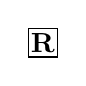
\begin{tikzpicture}\node [draw,shape=rectangle,inner sep=1pt] {\rule[-0.7pt]{0pt}{8.4pt}$\mathbf{R}$};\end{tikzpicture}}\hspace{1pt}}

\newcommand{\shared}[1]{{\fboxsep=0.4pt\fbox{\ensuremath{\;\begin{array}{@{}r@{}}#1\end{array}\;}}\hspace{1pt}}}
\newcommand{\Fshare}[3]{\shared{#1}^{#2}_{#3}}
\newcommand{\shareds}[1]{{\fboxsep=1pt\fbox{\ensuremath{{\phantom{||}\!\!\!}#1\,}}\hspace{1pt}}}
\newcommand{\Fshares}[3]{\shareds{#1}^{#2}_{#3}}

\newcommand{\actquant}{\exists}
\newcommand{\actto}{\leadsto}
\newcommand{\actap}[5]{#1 (#2) : \ \actquant #3 \ldotp \left({#4} \actto {#5}\right)}
\newcommand{\acta}[4]{#1 (#2) : \ {#3} \actto {#4}}
\newcommand{\actan}[3]{#1 : \ {#2} \actto {#3}}
\newcommand{\actanp}[4]{#1 : \ \actquant #2 \ldotp \left({#3} \actto {#4}\right)}

\newcommand{\Fall}{\mathrm{all}}
\newcommand{\Fperm}[4]{\left[ #1 ( #2 ) \right]^{#3}_{#4}}
\newcommand{\Fpermn}[3]{\left[ #1 \right]^{#2}_{#3}}

\newcommand{\upimp}{\mathop{\equiv \mspace{-3mu} \Rrightarrow}}
\newcommand{\Fupimp}[2]{\upimp^{\{#1\}\{#2\}}}

\newcommand{\Fup}[2]{\left[ \frac{#1}{#2} \right>}


% Rank-r characteristic of a world
\newcommand{\charac}[2]{D^{#1}_{#2}}
